% 
% setwd("/home/triffe/git/EquilateralLexis/EquilateralLexis/Draft2")
% Sweave("/home/triffe/git/EquilateralLexis/EquilateralLexis/Draft2/EquilateralLexis.Rnw")
% system("pdflatex EquilateralLexis.tex")
\documentclass[a4paper]{article}
\usepackage{amsmath}
\usepackage{natbib}
\bibpunct{(}{)}{,}{a}{}{;} 
\usepackage{url}
\usepackage{graphicx}
\usepackage{color}
\usepackage{epsfig}
\usepackage{float}
\usepackage{subfigure} 
\usepackage{verbatim}
\usepackage[OT1]{fontenc}
\usepackage{Sweave} % can be removed if submitted as latex file

\defcitealias{HFD2011}{HFD, 2011}
\defcitealias{wilmoth2007methods}{Wilmoth et. al., 2007}

\begin{document}

\title{(Re)introducing the equilateral age-period-cohort demographic surface}
\author{Tim Riffe \\ Department of Demography \\ University of California, Berkeley}
\maketitle

\thispagestyle{empty} % remove page numbering
\pagestyle{empty}

\vspace{2cm}

\begin{abstract}
The use of demographic surfaces based on time proportionality between age, period, and cohort axes is introduced as an alternative to standard \textit{Lexis} proportions in order to eliminate distortion of the cohort perspective and ensure comparable time scales. Resulting images are legible and interpretable in a similar way to standard demographic surfaces, but entail no visual bias in the visual comparison of slopes between temporal dimensions.
\end{abstract}

\pagebreak

This paper is about demographic data visualization and the link between the \textit{Lexis}\footnote{in italics throughout because Wilhelm Lexis was only one of many potential namesakes \citep{vandeschrick2001lexis, keiding2011age}} diagram and demographic surfaces. Any demographic quantity cross-classified by age, period and cohort (APC), or any two thereof, is candidate to be plotted as a demographic surface. Usually, such a surface is projected onto an age-period cartesian grid, with age on the $y$ axis and calendar year on the $x$ axis. The plane is then filled with color gradients or contour lines to specify value intervals for the quantity in question, the third dimension. It may be a misnomer to refer to such figures as surfaces, since these do not create an illusion of three-dimensionality (as per a stereogram or perspective plot) but the analogy invites the use of one's spatial intuition in understanding the data. This family of demographic plot is a subset of heatmaps or contour plots.\footnote{Edmund Halley is often cited as the maker of the first contour map (an isogonic map), and he also holds a place in the history of demography for the development of lifetables.} One of the main points of plotting a demographic surface is to view data over all three major time axes. The demographer often searches for cohort patterns in the data, diagonal ridges or trend shifts, that would be less apparent if viewed as a series of lines along the age or period year dimensions.

Demographic surfaces are almost always rendered following the cartesian time-axis conventions of the \textit{Lexis} diagram, which forces a unity aspect ratio between calendar years and age years along the age and time axes. Cohorts are represented by diagonal lines at 45$^\circ$, where a single cohort year stretches across the hypotenuse of the standard Lexis triangle, making it around 40\% longer on paper than an age or calendar year. While unproblematic in didactic line diagrams, this cohort distortion can cause visual bias when comparing the period and cohort dimensions of data. I reintroduce a coordinate transform that ensures a 1:1:1 relationship between all three temporal dimensions in the APC surface, thereby aiding visual interpretation of surfaces. This is the same graphical relationship originally rendered by Lexis as a diagram, and thereafter in the famous stereogram of Luigi Perozzo (1879), but never applied to the graphical representation of demographic data in contemporary graphics.

\subsection*{Cohort distortion in the \textit{Lexis} diagram}
The \textit{Lexis} diagram conforms to a set of principles on orientation and proportionality, including a unity aspect ratio between age increasing upward on the y-axis and calendar years increasing rightward along the x-axis. A unity aspect ratio means that one year in the age direction is equal to one year in the period direction when drawn. Birth cohorts start with years on the x axis at age 0 and increase upward and to the right at a 45$^\circ$ angle (segment AC). Imaginary life lines of individuals within the population follow along the cohort direction. A side effect of this 45$^\circ$ angle is that the cohort dimension is stretched on paper by about 40\% (scaled by $\sqrt{2}$). Demographers are well aware of this distortion, but it does not make the \textit{Lexis} diagram any less useful.\footnote{For example, the HMD Methods Protocol \citepalias{wilmoth2007methods} makes explicit mention of the $\sqrt{2}$ distortion of the cohort dimension in diagrams.}\\ 

These conventions conform to demographers' 'data-intuition', as demographic data are typically collected annually, and the most-used indicators are period indicators. A clear right angle between period and age lends itself to illustrating period indicators. Resulting cohort dimension distortion is largely innocuous when drawn as a diagram in outline form, since \textit{Lexis} diagrams do not represent data values, but rather data structure and relations. Distortion only arises when plotting data values represented by color gradients, contour lines, or similar graphical devices. To illustrate the nature of this bias, consider a line graph, for instance a log mortality curve over age. Figure~\ref{Fig0} shows US year 2010 log male mortality \citepalias{wilmoth2007methods}, with the principle axis on the bottom. The stretched axis on the top represents the exact degree of distortion that the cohort dimension is subject to on Lexis surfaces. From this it is clear that the nature of this distortion impedes the visual judgement of slopes, but not levels. 

\begin{figure}[ht!]
\centering
\caption{Translation of the visual bias in the standard \textit{Lexis} surface.}
\label{Fig0}
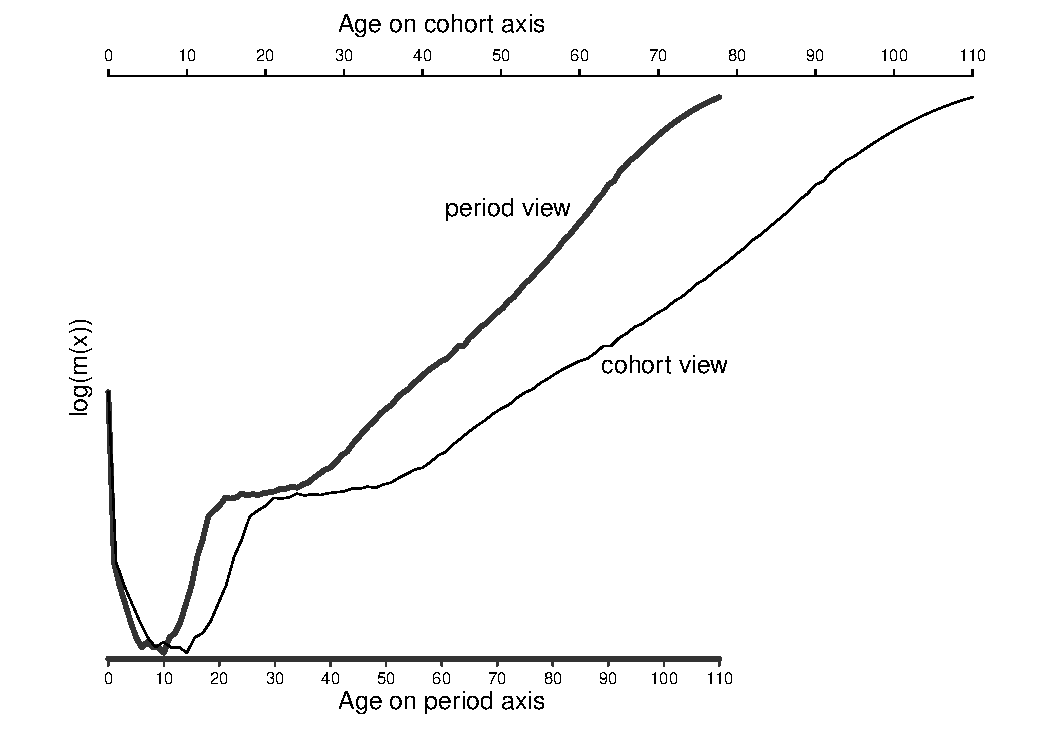
\includegraphics[width=7cm,height=5cm]{Figs/LineGraph.pdf}
\end{figure} 

Modern computing has facilitated the visualization of large tables of demographic rates cross-classified by age, period and cohort using surface plots, an idea popularized by \citet{arthur1984some}. Software packages have been designed to do this with demographic data, such as \texttt{LEXIS} by \citet{vaupel1987thousands} or the \texttt{Lexis} program by \citet{andreev1999overview}, which recognize and graphically represent the inherent triple-classification of the underlying data. A variety of general surface functions for gridded data (e.g., age-period only) in widely used statistical programming languages\footnote{such as \texttt{levelplot()} in the \texttt{lattice} package \citep{sarkar2008lattice} for gridded data in the R language \citep{ihaka1996r}, or the \texttt{contourf()} function in \texttt{MATLAB} \citep{MATLAB2010}, among many others.} that can be coerced to accurately represent standard demographic surfaces. Surface plots produced in this lineage have followed the design principles of the \textit{Lexis} diagram, entailing distortion of the cohort dimension in favor of a right angle between the age and period dimensions.\footnote{Rearranging the data, a less common rendering of age in the y-axis and cohort in the x-axis with a unity aspect ratio, in which case the period dimension is stretched by the same amount.}

Surface plots are about summarizing data; the human eye can find patterns and relationships in the data when represented as a surface. Demographic surfaces are a diagnostic tool, but more importantly they offer tremendous potential to illustrate and inspire stories from the data that aid understanding, and that can even sometimes make intuitive difficult-to-grasp concepts, such as tempo and quantum. The utility of demographic surface plots is therefore different from but complimentary to that of \textit{Lexis} diagrams. Cohort distortion in surfaces is at times a problem because the viewer is implicitly invited to judge the three temporal perspectives.

\subsection*{An equilateral coordinate system}
One can ensure visual comparability between the age, period and cohort perspectives by mapping data to equilateral triangles rather than to \textit{Lexis} right triangles. In this way, one year older in the age direction is equal to one year lived in the cohort direction and one calendar year in the period direction. Under this system, age-period squares become age-period diamonds\footnote{60-120 degree rhombuses}, and so forth. The idea of using equilateral triangles to ensure proportionality in APC renderings is not new. \citet{lexis1875einleitung} first entertained the use of 60$^\circ$ angles\footnote{See \citet{lexis1875einleitung} page 13, and Figure 2}, later developed by \citet{lewin1876rapport} and implemented in the famous stereogram of \citet{perozzo1880della}\footnote{At the time of this writing I have been unable to locate \citet{lewin1876rapport}, but it is included in the discussion by \citet{keiding2011age}.}. The present proposal for rendering such a surface is in keeping with the present-day convention of age increasing upward, rather than downward.\\

The arithmetic required to transform standard \textit{Lexis} surface coordinates into equilateral coordinates on a cartesian plane while maintaining a 1:1 scale is straightforward. Using $p$ to denote year, $a$ for age and $c$ for cohort, we can produce x and y coordinates for the standard and equilateral triangles seen in Figure~\ref{Fig1}. Figure~\ref{Fig1} compares a diagram of age-period regions (any given $p$ and $a$) divided into two APC triangles using the standard \textit{Lexis} proportions (left) and an equilateral proportions (right). Points A, B, C and D map to each other in both depictions.\\

\begin{figure}[ht!]
\centering
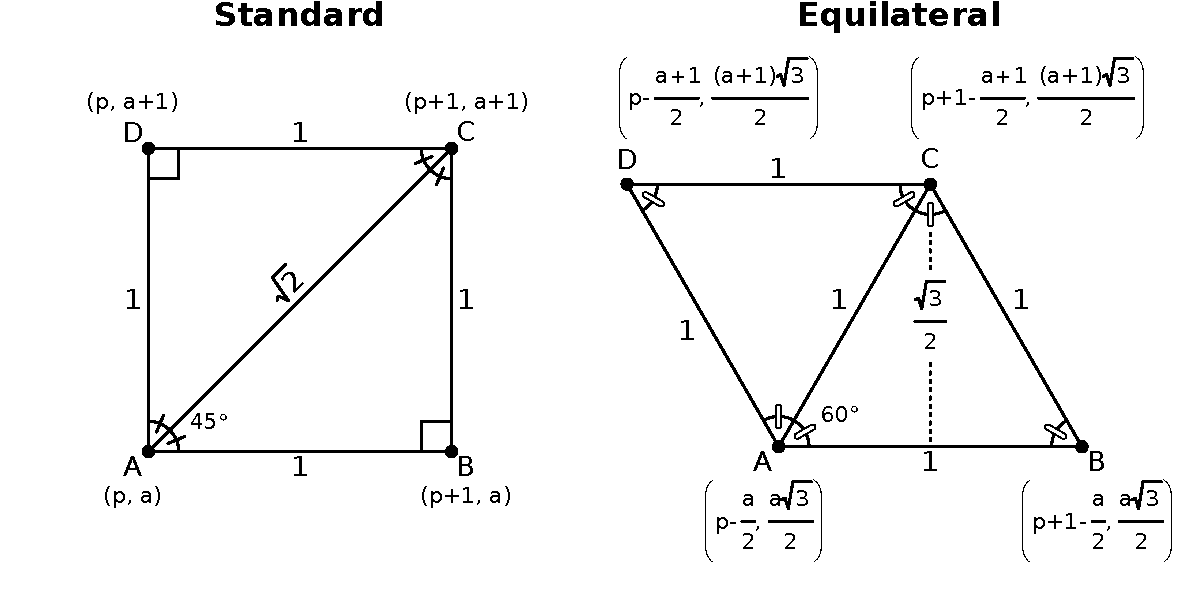
\includegraphics[width=12cm,height=6cm]{Figs/Figure1.pdf}
\caption{Standard \textit{Lexis} versus equilateral coordinates.}
\label{Fig1}
\end{figure}

The segment AD marks the beginning of year $p$, and BC marks year $p+1$ in both diagrams. In the equilateral depiction, however, years slant upward and to the left at 120$^\circ$. The age dimension is read horizontally in both depictions, segments AB ($a$) and DC ($a+1$), and its length remains 1. Segment AC marks cohort $c$ in both depictions, dividing the upper triangle ACD (when $p-c-a=1$) from the lower triangle ABC (when $p-a=c$). Segment AC changes its angle from 45$^\circ$ in the standard depiction to 60$^\circ$ in the equilateral depiction. Importantly, its length changes from $\sqrt{2}$ in the standard drawing to 1 in the equilateral drawing, which is the entire justification for this transform.\\ 

In short, to translate from standard to equilateral \textit{Lexis} coordinates for any given $(p,a)$ pair, subtract $\frac{a}{2}$ from $p$ and scale $a$ by $\frac{\sqrt{3}}{2}$ (or $\sin{60^\circ}$).

\subsection*{Standard versus equilateral APC demographic surfaces}
A demographic surface composed of tessellating APC equilateral triangles (or AP, PC or AC diamonds) is not radically different or exotic from one made of the more commonly used APC \textit{Lexis} triangles (or AP squares, or PC or AC parallelograms); it appears slanted 30$^\circ$ to the left, rather than as a rectangular surface. Compare two renderings of Czech APC fertility rates extracted from the Human Fertility Database \citepalias{HFD2011} in Figure~\ref{Fig2}.\\

The equilateral demographic surface in Figure~\ref{Fig2} resembles the better-known standard demographic surface closely enough that one generally familiar with interpreting surfaces requires little effort to understand it equally well. For this particular Czech fertility surface, one appreciates the visual transform of the post-velvet revolution fertility changes (say, from 1992 to 2005) in the equilateral rendition. The 1975 cohort, for instance, stands  in relatively sharp relief against the 1974 cohort in the age range 17 to 23 in both the standard and equilateral forms, but its relative importance (say, relative to the year 2000 ASFR) can be assessed with fidelity only in the later. The same advantage holds for each inter-cohort postponement decrease in the age-range 17-23 in the 1974-1977 cohorts, and for inter-cohort fertility increases above age 30 in the 1969-1977 cohorts (and potentially beyond). Period shifts, such as 1964-1965 or 1979-1980 are just as eye-catching in the equilateral surface as they are when viewed at 90$^\circ$ in the standard surface. On the whole, the equilateral surface from Figure~\ref{Fig2} enhances one's understanding of the underlying data.

\begin{figure}[H]
\centering
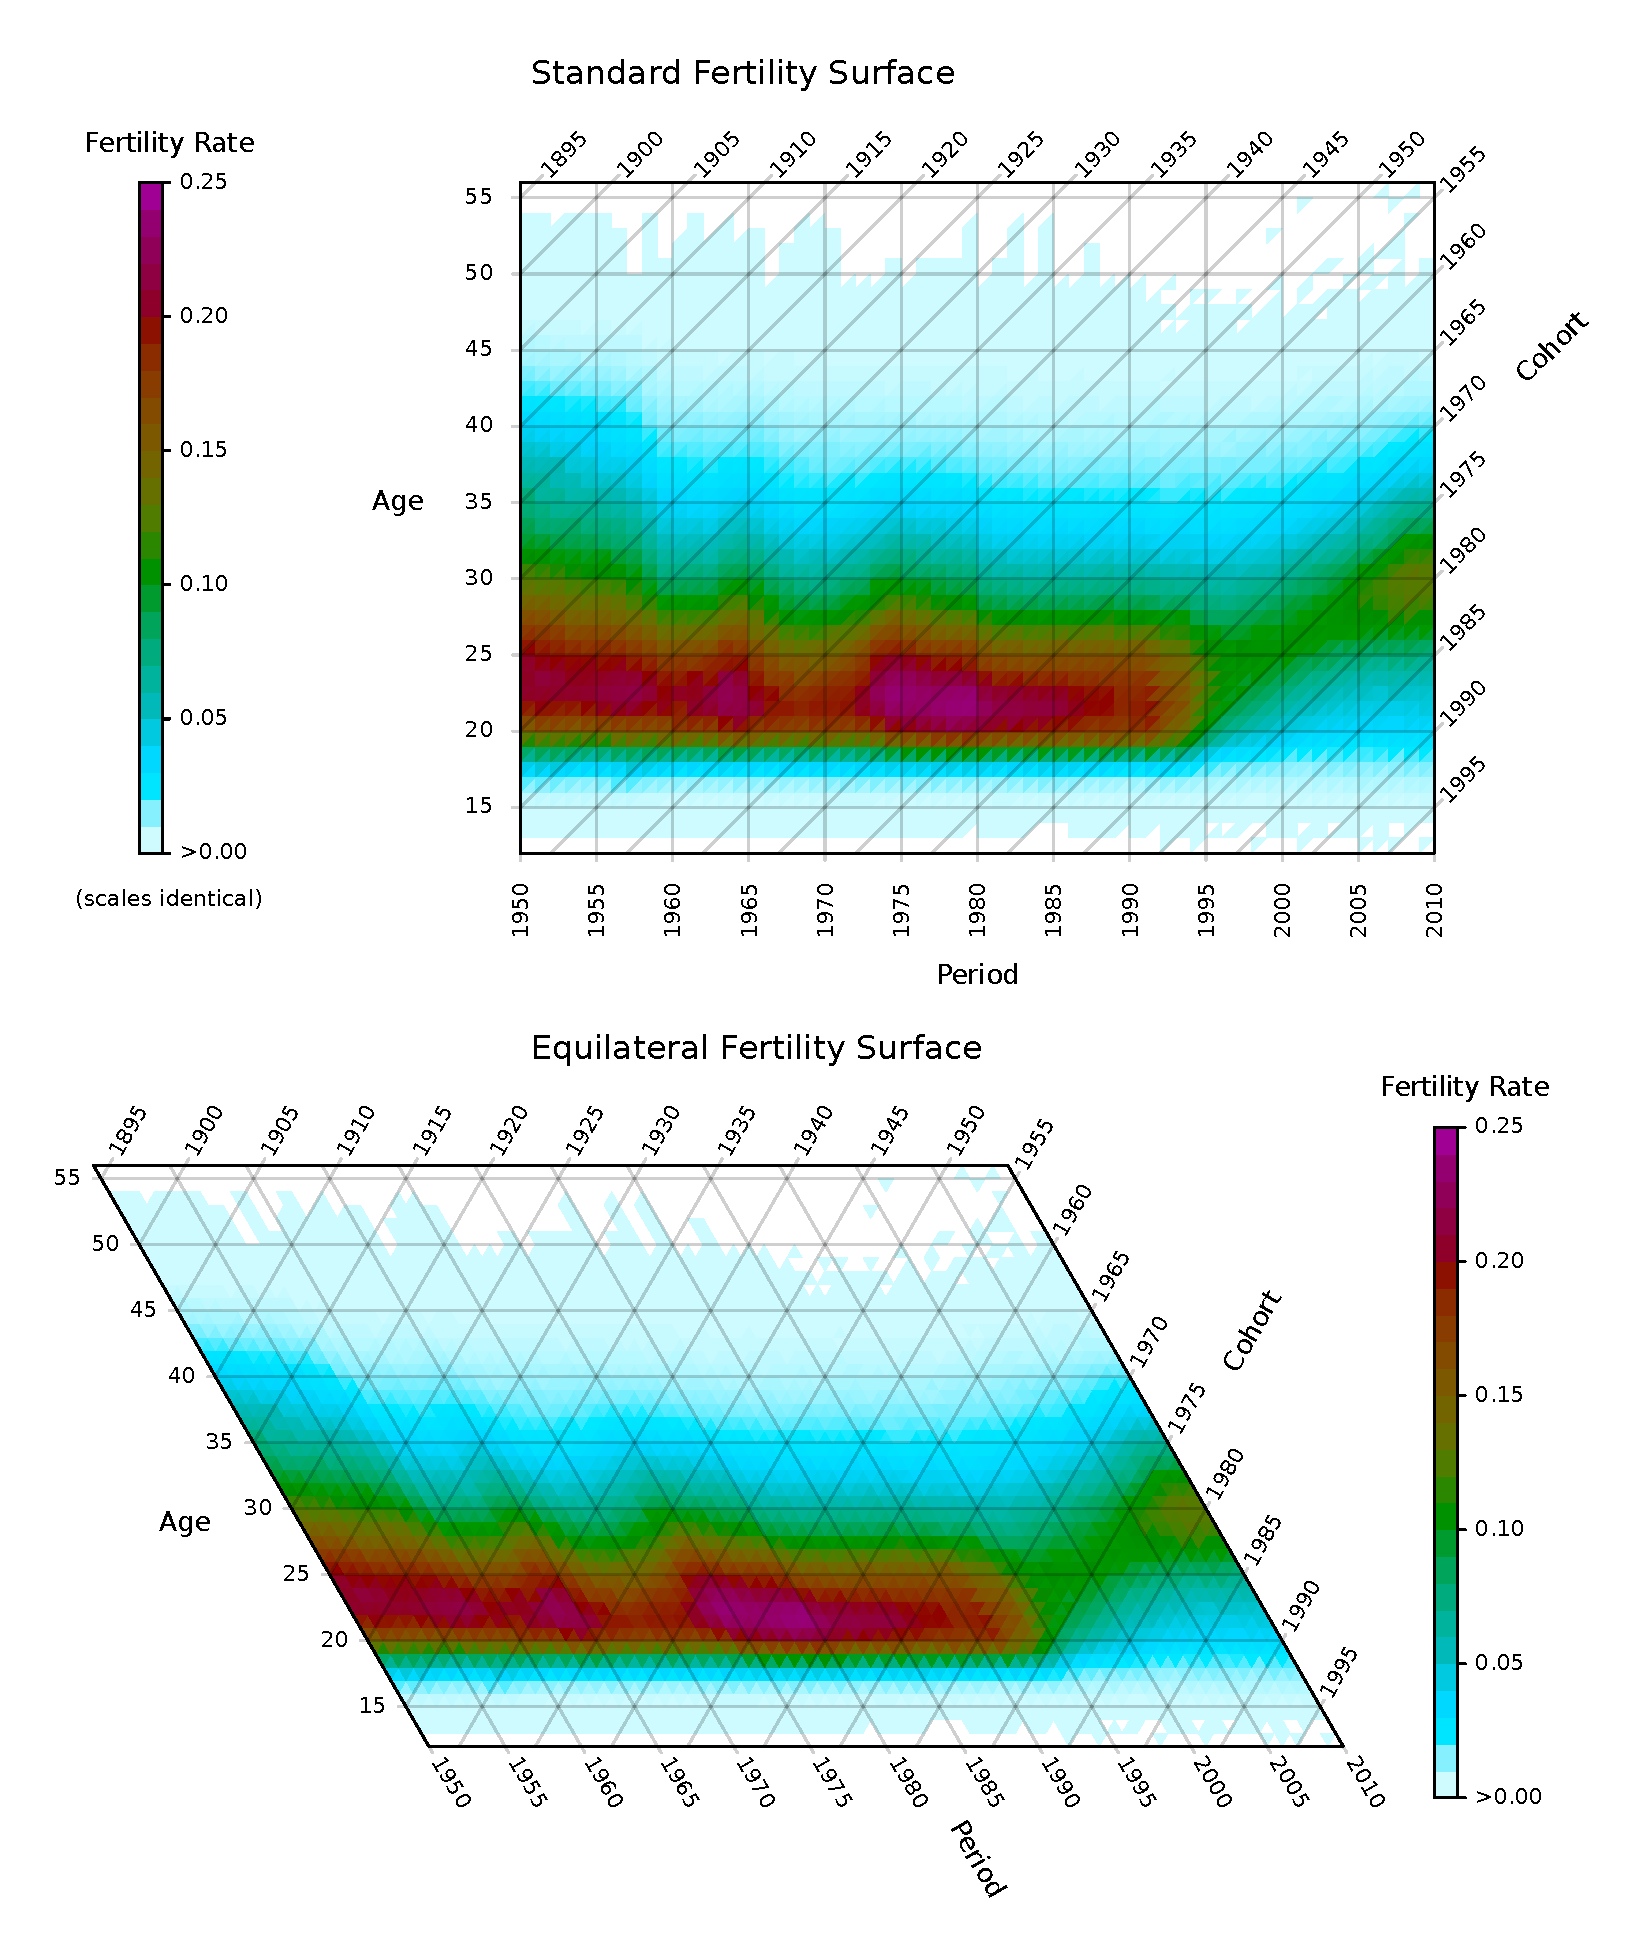
\includegraphics[width=16.5cm,height=19.5cm]{Figs/Figure2HCLd.pdf}
\caption{Czech Age-Period-Cohort specific fertility rates, 1950-2009 (HFD). Standard \textit{Lexis} proportions and coordinates (above) versus equilateral (below). Surfaces are plotted on 1:1 scales and share the same color legends and value intervals.}
\label{Fig2}
\end{figure}
 
The color scale used in Figure~\ref{Fig2} also adds value by interpolating over the HCL color space \citep{ihaka2003colour, colorspace2011} rather than the more frequently used RGB or HSV color spaces, either of which would entail irregularly perceived color intensity, potentially leading to false edges or other optical illusions \citep{zeileis2009escaping}. This HCL ramp equalizes perceived distance between colors by forcing a uniform colorfulness (chroma) and equidistant hues. An approximately linear luminance gradient ensures that the surface remains intelligible, albeit less sharp, both for color blind viewers and on grey scale devices. Further work is needed to establish best practices for the use of color in demographic surfaces in general and the most frequently used subtypes of APC surfaces, i.e. mortality and fertility, in particular.

\subsection*{Conclusions}
Equilateral Lexis surfaces overcome the problem of cohort distortion found in standard APC surfaces, and they are worth consideration for use in both diagnostic and didactic settings, minimally for the sake of comparison. The small tweak to the cohort dimension that sparked this endeavor has not been overlooked in recent applications of \textit{Lexis} diagrams, but the coordinate transform presented here appears never to have been implemented for APC demographic surfaces. The R code used to create the surfaces in Figure~\ref{Fig2} is freely available in the online appendices to this paper, and an R package for making both standard and equilateral demographic surfaces is currently in preparation.

\bibliographystyle{plainnat}
\bibliography{References.bib}   

\end{document}
